\documentclass[12pt, leqno]{article} %% use to set typesize
\input{common}

\usepackage{fontspec}
\usepackage{polyglossia}
\setmonofont{DejaVu Sans Mono}[Scale=MatchLowercase]
\usepackage[outputdir=pdf]{minted}

\providecommand{\tightlist}{%
  \setlength{\itemsep}{0pt}\setlength{\parskip}{0pt}}
\begin{document}



\hdr{2023-05-01}

\section{Lay of the Land}

In the landscape of continuous optimization problems, there are three
ways for things to be hard:

\begin{itemize}
\tightlist
\item
  Lack of smoothness
\item
  Lack of convexity (or other structure guaranteeing unique global
  minimizers)
\item
  Lack of information about the function
\end{itemize}

So far, we have only considered difficulties associated with lack of
convexity, and those only superficially -- most of our algorithms only
give local minimizers, and we haven't talked about finding global
optima. We have assumed everything has as many derivatives as we would
like, and that we are at least able to compute gradients of our
objective.

Today we discuss optimization in one of the hard cases. For this class,
we will not deal with the case of problems with very hard global
structure, other than to say that this is a land where heuristic methods
(simulated annealing, genetic algorithms, and company) may make sense.
But there are some useful methods that are available for problems where
the global structure is not so hard as to demand heuristics, but the
problems are hard in that they are ``black box'' -- that is, we are
limited in what we can compute to looking at function evaluations.

Before describing some methods, I make two pleas.

First, consider these only after having thoughtfully weighed the pros
and cons of gradient-based methods. If the calculus involved in
computing the derivatives is too painful, consider a computer algebra
system, or look into a tool for automatic differentiation of computer
programs. Alternately, consider whether there are numerical estimates of
the gradient (via finite differences) that can be computed more quickly
than one might expect by taking advantage of the structure of how the
function depends on variables. But if you really have to work with a
black box code, or if the pain of computing derivatives (even with a
tool) is too great, a gradient-free approach may be for you.

Second, do not fall into the trap of thinking these methods should be
simple to implement. Nelder-Mead is perhaps simple to implement, which
is one reason why it remains so popular; it also fails to converge on
many examples, and rarely converges fast. There are various pattern
search methods and model-based methods with more robust convergence or
better convergence rates, and there exist good implementations in the
world (though Powell himselff has passed, his
\href{https://www.pdfo.net/}{PDFO suite} is still going strong!). And
there are much more thorough texts and reviews than this set of lecture
notes; a few I like include:

\begin{itemize}
\tightlist
\item
  \href{https://doi.org/10.1017/S0962492900002841}{Powell, ``Direct
  search algorithms for optimization calculations''} -- covers a lot of
  methods, and particularly Powell's algorithms
\item
  \href{http://www.damtp.cam.ac.uk/user/na/NA_papers/NA2007_03.pdf}{Powell,
  ``A view of algorithms for optimization without derivatives''} --
  played a big role in this presentation
\item
  \href{https://epubs.siam.org/doi/10.1137/S003614450242889}{Kolda,
  Lewis, and Torczon, ``Optimization by direct search: new perspectives
  on some classical and modern methods''} -- deals with one interesting
  family of methods (very thoroughly)
\item
  \href{https://epubs-siam-org.proxy.library.cornell.edu/doi/book/10.1137/1.9780898718768}{Conn,
  Scheinberg, and Vicente, ``Introduction to Derivative-Free
  Optimization''} -- available for access via the Cornell library
  subscription to SIAM ebooks
\item
  \href{https://link-springer-com.proxy.library.cornell.edu/book/10.1007/978-3-319-68913-5}{Audet
  and Warren, ``Derivative-Free and Blackbox Optimization''} -- a
  Springer textbook, but also available courtesy the Cornell library
\item
  \href{https://arxiv.org/pdf/1904.11585.pdf}{Larson, Menickelly, and
  Wild, ``Derivative-free optimization methods''} -- a recent Acta
  Numerica survey, again by people who know what they are doing
\end{itemize}

\section{Model-based methods}

The idea behind Newton's method is to successively minimize a quadratic
\emph{model} of the function behavior based on a second-order Taylor
expansion about the most recent guess, i.e.~\(x^{k+1} = x^k + p\) where
\[\operatorname{argmin}_{p} \phi(x) + \phi'(x) p + \frac{1}{2} p^T H(x) p.\]
In some Newton-like methods, we use a more approximate model, usually
replacing the Hessian with something simpler to compute and factor. In
simple gradient-descent methods, we might fall all the way back to a
linear model, though in that case we cannot minimize the model globally
-- we need some other way of controlling step lengths. We can also
explicitly incorporate our understanding of the quality of the model by
specifying a constraint that keeps us from moving outside a ``trust
region'' where we trust the model to be useful.

In derivative-free methods, we will keep the basic ``minimize the
model'' approach, but we will use models based on interpolation (or
regression) in place of the Taylor expansions of the Newton approach.
There are several variants.

\subsection{Finite difference derivatives}

Perhaps the simplest gradient-free approach (though not necessarily the
most efficient) takes some existing gradient-based approach and replaces
gradients with finite difference approximations. There are a two
difficulties with this approach:

\begin{itemize}
\tightlist
\item
  If \(\phi : \mathbb{R}^n \rightarrow \mathbb{R}\), then computing the
  \(\nabla \phi(x)\) by finite differences involves at least \(n+1\)
  function evaluations. Thus the typical cost per step ends up being
  \(n+1\) function evaluations (or more), where methods that are more
  explicitly designed to live off samples might only use a single
  function evaluation per step.
\item
  The finite difference approximations depends on a step size \(h\), and
  their accuracy is a complex function of \(h\). For \(h\) too small,
  the error is dominated by cancellation, revealing roundoff error in
  the numerical function evaluations. For \(h\) large, the error depends
  on both the step size and the local smoothness of the function.
\end{itemize}

The first issue (requiring \(n+1\) function evaluations to get the same
information content as one function-and-gradient evaluation) is not
unique to finite difference computations, and indeed tends to be a limit
to a lot of derivative-free methods.

\subsection{Linear models}

A method based on finite difference approximations of gradients might
use \(n+1\) function evaluations per step: one to compute a value at
some new point, and \(n\) more in a local neighborhood to compute values
to estimate derivatives. An alternative is to come up with an
approximate linear model for the function using \(n+1\) function
evaluations that may include some ``far away'' function evaluations from
previous steps.

We insist that the \(n+1\) evaluations form a simplex with nonzero
volume; that is, to compute from evaluations at points
\(x_0, \ldots, x_n\), we want \(\{ x_j-x_0 \}_{j=1}^n\) to be linearly
independent vectors. In that case, we can build a model
\(x \mapsto b^T x + c\) where \(b \in \mathbb{R}^n\) and
\(c \in \mathbb{R}\) are chosen so that the model interpolates the
function values. Then, based on this model, we choose a new point.

The following routine computes a simplex estimate
\(\hat{\nabla} f(x_0)\) of the gradient \(\nabla f(x)\) based on the
equations \[f(x_i) = f(x_0) + (x_i-x_0)^T \hat{\nabla} f(x_0),\] Our
gradient estimator therefore has the form
\[A \hat{\nabla} f(x_0) = y, \quad 
  A = \begin{bmatrix} (x_1-x_0)^T \\ \vdots \\ (x_n-x_0) \end{bmatrix}, \quad
  y = \begin{bmatrix} f(x_1) - f(x_0) \\ \vdots \\ f(x_n)-f(x_0) \end{bmatrix}.\]
Note that if we adapt the simplex by changing one point at a time, we
can update the factorization of \(A\) in \(O(d^2)\) time rather than
recomputing every time at a cost of \(O(d^3)\). We do not bother to do
this here, though.

\begin{minted}{julia}
function simplex_gradient(xs, fxs)
    d, np1 = size(xs)
    A = (xs[:,2:end].-xs[:,1])'
    ∇f_s = A\(fxs[2:end].-fxs[1])
    ∇f_s, cond(A)
end
\end{minted}

The true gradient satisfies \[A \nabla f(x_0) = y + r;\] where the
vector \(r\) consist of remainder terms from Taylor's theorem with
remainder. If the gradient is Lipschitz with constant \(M\), then the
terms satisfy \[r_i \leq M \|x_i-x_0\|^2/2 \leq M d^2/2\] where \(d\) is
the diameter of the simplex. Therefore, we expect
\[\|\hat{\nabla} f(x_0) - \nabla f(x_0)\| \leq 
  \|A^{-1} r\| \leq \|(A/d)^{-1}\| Md/2\] where \(\|(A/d)^{-1}\|\) is
scaled so that only the geometry of the simplex matters. Alternately, we
have the relative error bound
\[\frac{\|\hat{\nabla} f(x_0) - \nabla f(x_0)\|}{\|\nabla f(x_0)\|} \leq 
  \kappa(A) \frac{Md}{2\|y\|/d}\] However we write the bounds, a key
aspect to these methods is ensuring that the computation of the affine
function from the simplex remains well-conditioned.

\begin{figure}
\begin{center}
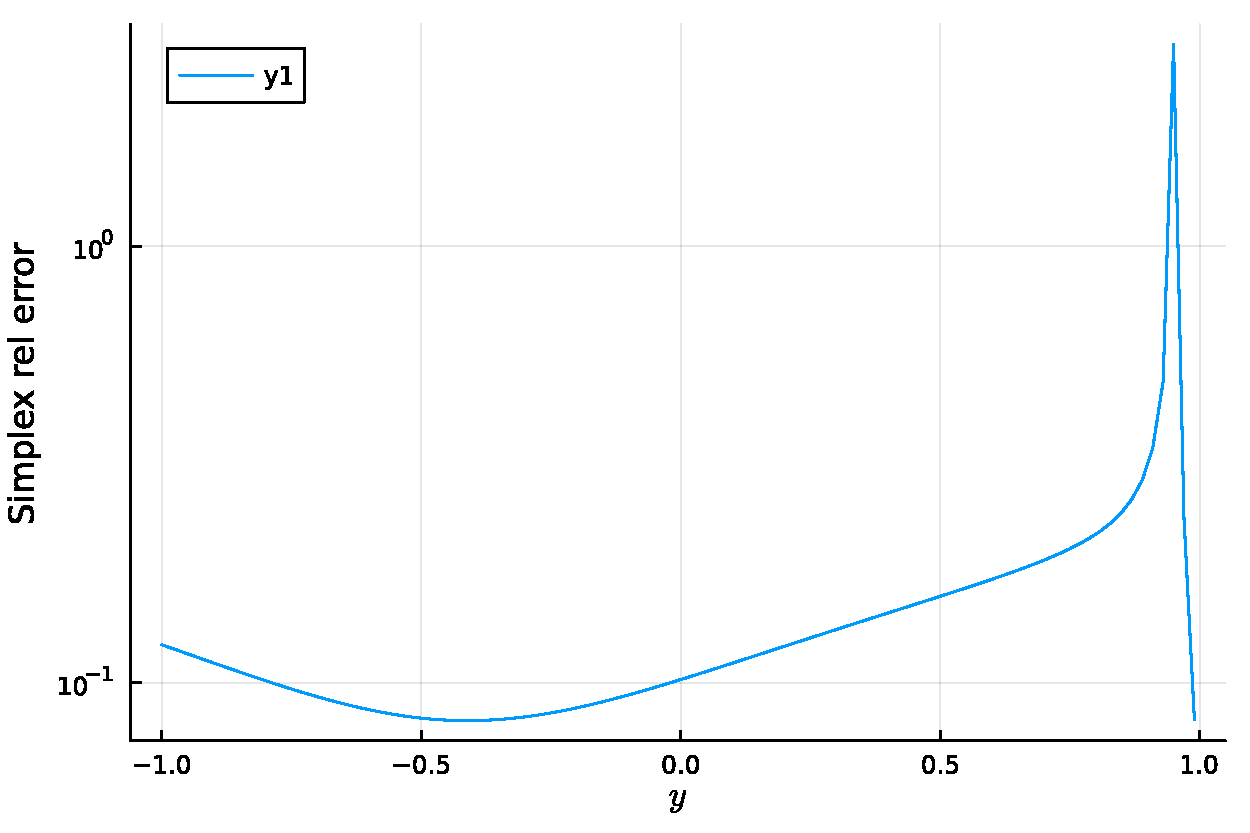
\includegraphics[width=0.8\textwidth]{fig/2023-05-01-simplex-err.pdf}
\end{center}
\caption{Simplex gradient estimate error.  As $y$ approaches 1, the simplex
  approaches degeneracy (and the linear system we have to solve approaches
  singularity).}
\label{fig:simplex-err}
\end{figure}

We give an example of the effects of geometry below by using a simplex
gradient approximation of a 2D function where we make the simplex closer
and closer to degenerate.  As we get closer to degenerate, the error in
the gradient estimate increases (Figure~\ref{fig:simplex-err}).

Getting a good gradient estimate gives a sense of which way to go, but
in order to get good convergence we also need a globalization strategy,
which gets more complicated. For example, line search with sufficient
decrease can fail because of an inaccurate gradient estimate, in which
case we may need to reconstruct a new simplex with a good geometry and a
small diameter. There are also trust-region methods that use linear
approximations based on interpolation over a simplex. One of the most
popular of this family of method is Powell's COBYLA algorithm
(Constrained Optimization BY Linear Approximation).

\subsection{Quadratic models}

One can build quadratic models of a function from only function values,
but to fit a quadratic model in \(n\)-dimensional space, we usually need
\((n+2)(n+1)/2\) function evaluations -- one for each of the
\(n(n+1)/2\) distinct second partials, and \(n+1\) for the linear part.
Hence, purely function-based methods that use quadratic models tend to
be limited to low-dimensional spaces. However, there are exceptions. The
NEWUOA method (again by Powell) uses \(2n+1\) samples to build a
quadratic model of the function with a diagonal matrix at second order,
and then updates that matrix on successive steps in a Broyden-like way.

\subsection{Surrogates and response surfaces}

Polynomial approximations are useful, but they are far from the only
methods for approximating objective functions in high-dimensional
spaces. One popular approach is to use \emph{kernel-based
approximations}; for example, we might write a model
\[s(x) = \sum_{j=1}^m c_j \phi(\|x-x_j\|)\] where the coefficients
\(c_j\) are chosen to satisfy \(m\) interpolation conditions at points
\(x_1, \ldots, x_m\). If we add a polynomial term, you'll recognize this
as the form of the interpolants from project 1, but the spline
interpretation is only one way of thinking about this class of
approximators. Another option is to interpret this as a Gaussian process
model; this is used, for example, in most Bayesian Optimization (BO)
methods. There are a variety of other surfaces one might consider, as
well.

In addition to fitting a surface that interpolates known function
values, there are also methods that use \emph{regression} to fit some
set of known function values in a least squares sense. This is
particularly useful when the function values have noise.

\section{Pattern search and simplex}

So far, the methods we have described are explicit in building a model
that approximates the function. However, there are also methods that use
a systematic search procedure in which a model does not explicitly
appear. These sometimes go under the heading of ``direct search''
methods.

\subsection{Nelder-Mead}

The Nelder-Mead algorithm is one of the most popular derivative-free
optimizers around. For example, this is the default algorithm used for
derivative free optimization with \texttt{Optim.jl}. As with methods
like COBYLA, the Nelder-Mead approach maintains a simplex of \(n+1\)
function evaluation points that it updates at each step. In Nelder-Mead,
one updates the simplex based on function values at the simplex corners,
the centroid, and one other point; or one contracts the simplex.

Visualizations of Nelder-Mead are often quite striking: the simplex
appears to crawl downhill like some sort of mathematical amoeba. But
there are examples of functions where Nelder-Mead is not guaranteed to
converge to a minimum at all.

\subsection{Hook-Jeeves and successors}

The basic idea of \emph{pattern search} methods is to either

\begin{itemize}
\tightlist
\item
  Keep going if a promising direction turns out good, or
\item
  Poll points in a pattern around the current iterate to find a new
  direction
\end{itemize}

For example, in the Hook-Jeeves approach (one of the earliest pattern
search methods), one would at each polling move evaluate
\(\phi(x^{(k)} \pm \Delta e_j)\) for each of the \(n\) coordinate
directions \(e_j\). If one of the new points is better than \(x^{(k)}\),
it becomes \(x^{(k+1)}\) (and we may increase \(\Delta\) if we already
took a step in this direction to get from \(x^{(k-1)}\) to \(x^{(k)}\).
Of \(x^{(k)}\) is better than any surrounding point, we decrease
\(\Delta\) and try again.

\begin{minted}{julia}
function hooke_jeeves(ϕ, x; Δ=1.0, Δtol=1e-3, maxevals=1000,
                      monitor=(x,Δ,poll)->nothing)

    ϕ0 = ϕ(x)     # Current best value found
    poll = true   # Poll step or keep going?
    evals = 0     # Number of function evaluations
    k = 0         # Current search direction

    # Possible search directions (+/- in each coordinate direction)
    d = length(x)
    P = [Matrix(I,d,d) -Matrix(I,d,d)]
 
    while Δ > Δtol && evals < maxevals
        monitor(x, Δ, poll)
        if poll

            # Poll in neighborhood.  Pick the best descent direction;
            # if we get no descent, cut the radius and try again.
            ϕPmin, kmin = findmin(ϕ(x + Δ*p) for p in eachcol(P))
            evals += 2*d
            if ϕ0 >= ϕPmin
                k = kmin
                poll = false
            else
                Δ = Δ/2
            end
 
        else

            # Take a step, accept if decrease, poll otherwise
            xnew = x + Δ*P[:,k]
            ϕnew = ϕ(xnew)
            evals += 1
            if ϕnew < ϕ0
                x[:] = xnew
                ϕ0 = ϕnew
            else
                poll = true
            end

        end
    end

    x, Δ
end
\end{minted}

\begin{figure}
\begin{center}
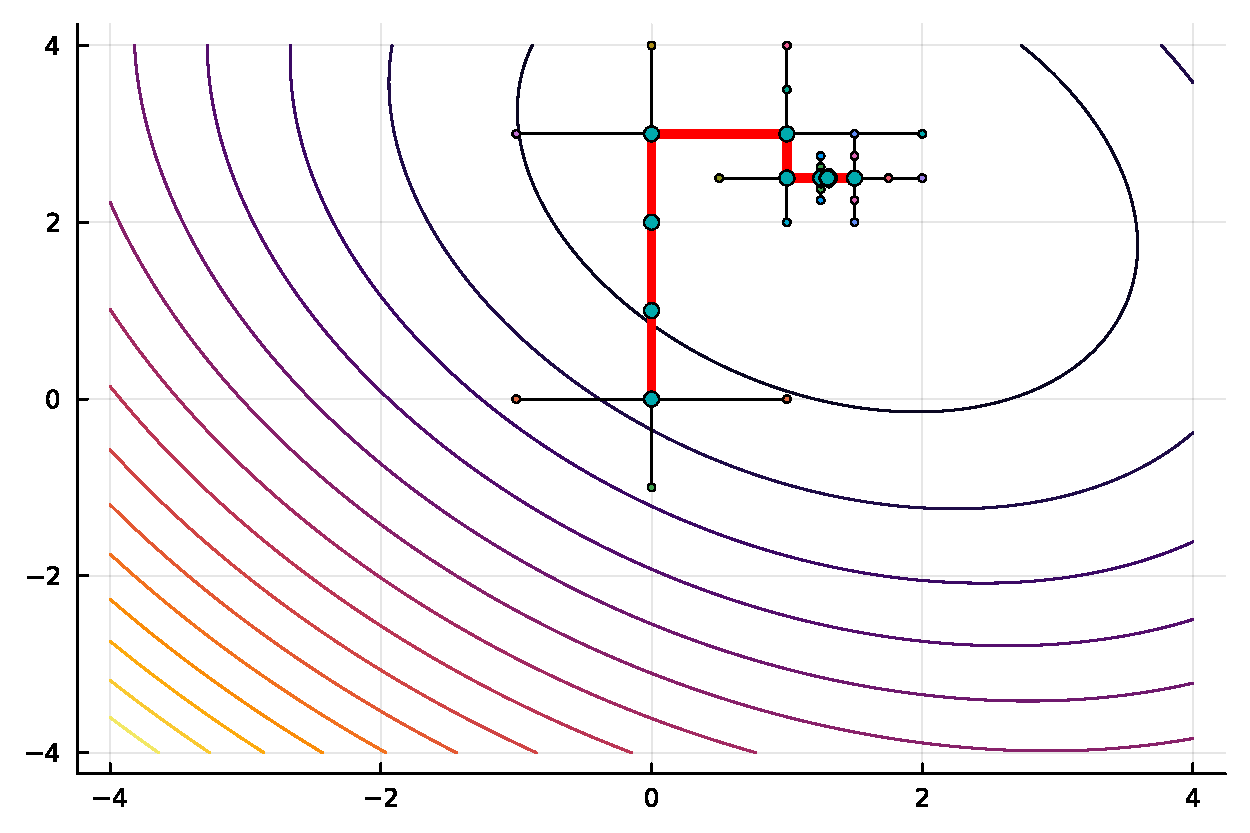
\includegraphics[width=0.8\textwidth]{fig/2023-05-01-hooke-jeeves.pdf}
\end{center}
\caption{Convergence of the Hooke-Jeeves algorithm for a quadratic
  model problem.}
\label{fig:hooke-jeeves}
\end{figure}

We give an example of the convergence of Hooke-Jeeves on a quadratic model
problem with the code below (Figure~\ref{fig:hooke-jeeves}).

More generally, we would evaluate \(\phi(x^{(k)} + d)\) for
\(d \in \mathcal{G}(\Delta)\), a \emph{generating set} of directions
with some scale factor \(\Delta\). There are many variants on the
``search-and-poll'' strategy of the general pattern search; for example,

\begin{itemize}
\tightlist
\item
  We can do a random selection from the pattern directions and choose
  the first promising one (rather than polling all directions).
\item
  We can use a model to suggest some extra promising directions in
  addition to the pattern, or to modify from a fixed pattern.
\end{itemize}

Simple methods like Hooke-Jeeves converge for smooth objectives, but may
fail in the nonsmooth case. However, the mesh adaptive direct search
(MADS) class of methods can converge even in this case.

\section{Summarizing thoughts}

Direct search methods have been with us for more than half a century:
the original Hook-Jeeves paper was from 1961, and the Nelder-Mead paper
goes back to 1965. These methods are attractive in that they require
only the ability to compute objective function values, and can be used
with ``black box'' codes -- or even with evaluations based on running a
physical experiment! Computing derivatives requires some effort, even
when automatic differentiation and related tools are available, and so
gradient-free approaches may also be attractive because of ease-of-use.

Gradient-free methods often work well in practice for solving
optimization problems with modest accuracy requirements. This is true
even of methods like Nelder-Mead, for which there are examples of very
nice functions (smooth and convex) for which the method is guaranteed to
mis-converge. But though the theoretical foundations for these methods
have gradually improved with time, the theory for gradient-free methods
is much less clear-cut than the theory for gradient-based methods.
Gradient-based methods also have a clear advantage at higher accuracy
requirements.

Gradient-free methods do \emph{not} free a user from the burden of
finding a good initial guess. Methods like Nelder-Mead and pattern
search will, at best, converge to local minima. Many heuristic methods
for finding global minimizers are gradient-free; I include among these
methods like simulated annealing, genetic algorithms, and Bayesian
optimization techniques. On the other hand, branch-and-bound methods
that yield provable global minimizers are often heavily dependent on
derivatives (or bounds proved with the help of derivatives).

Just because a method does not explicitly use gradients does not mean it
doesn't rely on them implicitly. Gradient-free methods may have just as
much difficulty with functions that are discontinuous, or that have
large Lipschitz constants -- particularly those methods that implicitly
build a local linear or quadratic model.

In many areas in numerics, an ounce of analysis pays for a pound of
computation. If the computation is to be done repeatedly, or must be
done to high accuracy, then it is worthwhile to craft an approach that
takes advantage of specific problem structure. On the other hand,
sometimes one just wants to do a cheap exploratory computation to get
started, and the effort of using a specialized approach may not be
warranted. An overview of the options that are available is useful for
approaching these tradeoffs intelligently.


\end{document}
